\skriptsection{Maximum-Likelihood and Bayesian Parameter Estimation}{84}

  \skriptsubsection{Maximum-Likelihood Estimation (ML)}{85}
  Maximum-Likelihood estimation tries to find an optimum solution if a parameter vector
  $\boldsymbol{\theta}$ is unknown.
  The likelihood of $\boldsymbol{\theta}$ with respect to the set of samples $\mathcal{D}$ is defined as 
  $p(\mathcal{D} | \boldsymbol{\theta}) = \prod_{k=1}^{n} p(\mathbf{x}_k | \boldsymbol{\theta})$ 
  (samples are i.i.d. - independent \& identically distributed).
  
  \begin{minipage}{12cm}
	  Recipe with log-likelihood: \\
	  \begin{tabular}{lll}
	  1. & Log-likelihood: & $l(\boldsymbol{\theta}) \equiv \ln (p(\mathcal{D} | \boldsymbol{\theta}))=\sum\limits_{k=1}^n \ln(p(\mathbf{x}_k | \boldsymbol{\theta}))$ \quad $\left( \frac{d}{dx} \ln(x) = \frac1x \right)$ \\
	  2. & Gradient: &  $\nabla_{\boldsymbol{\theta}} l = 
	  	      \sum\limits_{k=1}^n \nabla_{\boldsymbol{\theta}}\ln(p(\mathbf{x}_k | \boldsymbol{\theta}))$ \\
	  3. & $\nabla_{\boldsymbol{\theta}} l = 0$: & find solution 
	  	      $\boldsymbol{\hat{\theta}}=\arg\max\limits_{\boldsymbol{\theta}} l(\bm{\theta})$ \\
	  \end{tabular}
  \end{minipage}
  \begin{minipage}{8cm}
  	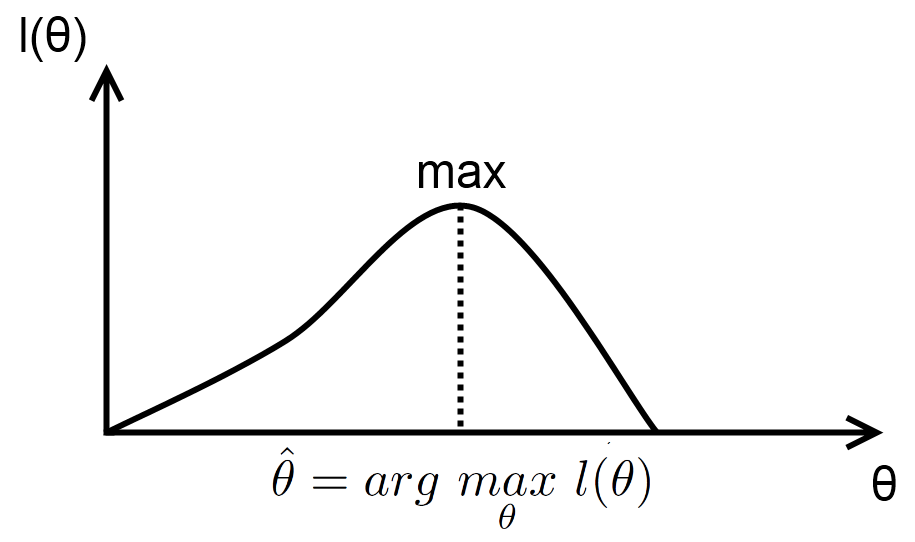
\includegraphics[width=7cm]{./images/MaxLikely.png}
  \end{minipage}
  
  The solution can be the true global maximum, a local maximum or minimum. Also check the boundaries of the parameter space for a possible maximum.
  \skriptsubsubsection{Gaussian case}{88}
  $\boldsymbol{\hat{\mu}} = \frac1n \sum\limits_{k=1}^n \mathbf{x}_k$ (called sample mean)\\
  $\boldsymbol{\hat{\Sigma}} = \frac1n \sum\limits_{k=1}^n 
  (\boldsymbol{x}_k - \boldsymbol{\hat{\mu}})(\boldsymbol{x}_k - \boldsymbol{\hat{\mu}})^T$ (called sample covariance)
  
  \skriptsubsubsection{Bias}{89}
  An estimation is biased if $E(\boldsymbol{\hat{\theta}}) \neq \theta$ or in words: if the expected 
  value of an estimation is not equal to the true value.
  E.g. the variance of a Gaussian distribution is biased.\\
  \subsubsubsection{Unbiased Estimator} of the variance is $\boldsymbol{C} = \frac1{n-1} \sum\limits_{k=1}^n 
  (\boldsymbol{x}_k - \boldsymbol{\hat{\mu}})(\boldsymbol{x}_k - \boldsymbol{\hat{\mu}})^T$ called sample covariance matrix.
  
  
  \skriptsubsection{Bayesian Estimation}{90}
  In Bayesian learning, we consider $\boldsymbol{\theta}$ to be a random variable and estimate the distribution of this variable.
  The main difference to the maximum-likelihood method is that we give to our guess for the $\boldsymbol{\hat{\mu}}$ and $\boldsymbol{\hat{\Sigma}}$ an 
   uncertainty\slash{}variance\slash{}distribution. Additionally the Bayes method can use prior knowledge. If there is such a prior knowledge Bayesian is possible 
   to reach the same result as ML with less training data. A disadvantage is, that it needs more calculating power, or better result with same training data, if the class-conditional density is known.
  
  \skriptsubsubsection{Class-Conditional Densities}{91}
  The heart of Bayesian classification: Computation of posterior probabilities. This is the 
  general formula:
  $$P(\omega_i|\bm{x}, \mathcal{D}) = \frac{p(\bm{x}|\omega_i, \mathcal{D}) P(\omega_i|\mathcal{D})}
    {\sum\limits_{j=1}^{c} p(\bm{x}|\omega_j, \mathcal{D}) P(\omega_j|\mathcal{D})}$$
    
    
  The assumption is that the prior probabilities are known or obtainable from a trivial calculation $P(\omega_i|\mathcal{D})=P(\omega_i)$.
  Furthermore, the training samples $\mathcal{D}_i$ now belong to categories $\omega_i$, 
  ($i=1\ldots,c$) and the samples of category $i$ are not influenced by category $j$ ($j \neq i$).
  Now, each category can be treated indepently.
  $$P(\omega_i|\bm{x}, \mathcal{D}) = \frac{p(\bm{x}|\omega_i, \mathcal{D}_i) P(\omega_i)}
    {\sum\limits_{j=1}^{c} p(\bm{x}|\omega_j, \mathcal{D}_j) P(\omega_j)}$$
    
  \skriptsubsubsection{Parameter Distribution}{91}
  We want to find the distribution of a parameter vector $\bm{\theta}$ for every class with a given dataset $\mathcal{D}$:
  $$\underbrace{p(\bm x |\omega_i)}_{\text{Likelihood}}\approx \underbrace{p(\bm{x}|\mathcal{D},\omega_i)}_{\text{Posterior}} = \int{p(\bm{x,\theta}|\mathcal{D}) d \theta}\overset{!*}{=}
  \underbrace{\int}_{\text{
  	\parbox{2.3cm}{\centering 
  		Multidimensional, hard to compute}}  
	}
  \underbrace{p(\bm{x}|\bm{\theta})}_{\text{Model}} 
  \underbrace{p(\bm{\theta}|\mathcal{D})}_{\text{given by training data}} d\bm{\theta}$$
 *: Because the selection of $\bm{x}$ and that of $\mathcal{D}$ is done independently.
  \skriptsubsubsection{Gaussian case: Univariate case}{92}
  with known $\sigma=\Sigma$. e.g. known measurement system but unknown measurement value\\
  \subsubsubsection{Finding the A Posteriori Density}
  \begin{aufzaehlung}
    \item Model: $p(x|\mu) \sim N(\mu, \sigma^2)$ ($\sigma^2$ is known)
    \item Goal: Finding $\mu$ as the only unknown parameter
    \item Best prior guess: $p(\mu) \sim N(\mu_0, \sigma_0^2)$
    \item Crucial assumption: Knowing the prior distribution of $\mu$ ($\mu$ is normal distributed).
    \item The Bayes formula is introduced: 
      $p(\mu|\mathcal{D}) = \frac{p(\mathcal{D}|\mu) p(\mu)}{\int p(\mathcal{D}|\mu) p(\mu) d\mu} = \frac{p(\mathcal{D}|\mu) p(\mu)}{p(\mathcal{D})}$
    \item And by forward calculation: 
      $p(\mu|\mathcal{D}) = \frac{1}{\sqrt{2\pi} \sigma_n} e^{-\frac12 (\frac{\mu-\mu_n}{\sigma_n})^2}$
      with $n$ as the number of samples (which can be increased). 
      $p(\mu|\mathcal{D})$ is called \em reproducing density \em and $p(\mu)$ is a \em conjugate prior \em.
    \item After some calculation, this results in
      $$\mu_n = (\frac{n\sigma_0^2}{n\sigma_0^2 + \sigma^2})\hat{\mu}_n + 
      \frac{\sigma^2}{n\sigma_0^2 + \sigma^2} \mu_0 \quad \text{ with } \quad
      \hat{\mu}_n = \frac1n \sum\limits_{k=1}^{n}x_k. \text{ (Sample Mean)}$$
      At the beginning ($n=0$), the initial value is weighted high ($\mu_0$) but with more samples
      the sample mean is weighted much higher ($\hat{\mu}_n$) and the initial knowledge is getting 
      unimportant when $n \rightarrow \infty$.\\
      The variance of the parameter distribution is
      $$\sigma_n^2 = \frac{\sigma_0^2 \sigma^2}{n\sigma_0^2 + \sigma^2}$$
      which leads to a Dirac delta function when $n \rightarrow \infty$.
  \end{aufzaehlung}
  
  \subsubsubsection{Finding the Class-Conditional Density}
  $$p(x|\mathcal{D}) = \int p(x|\mu) p(\mu|\mathcal{D}) d\mu \sim N(\mu_n, \sigma^2+\sigma_n^2)$$ 
    
  \skriptsubsubsection{Gaussian case: Multivariate case}{95}
  with known $\bm\Sigma$ but unknown $\bm{\mu}$.\\
  The generalization of the a posteriori calculation leads to:
  $$\bm{\mu}_n = \bm{\Sigma}_0 \Big(\bm{\Sigma}_0 + \frac1n \bm{\Sigma}\Big)^{-1}\bm{\hat{\mu}}_n +
    \frac1n \bm{\Sigma} \Big(\bm{\Sigma}_0 + \frac1n \bm{\Sigma}\Big)^{-1} \bm{\mu}_0,$$
  its variance
  $$\bm{\Sigma}_n = \bm{\Sigma}_0 \Big( \bm{\Sigma}_0 + 
    \frac1n \bm{\Sigma}\Big)^{-1}\; \frac1n{\bm{\Sigma}}$$
  
  and the class-conditional density is
  $$p(\bm{\mu}|\mathcal{D}) \sim N(\bm{\mu}_n, \bm{\Sigma} + \bm{\Sigma}_n)$$
  
  \skriptsubsubsection{Recursive Bayes Learning}{98}
  \em Bayesian learning \em can be done when the class-conditional density function is expressed 
  as recursive formula and it converges to a Dirac delta function:
  $$p(\bm{\theta} | \mathcal{D}^n) = \frac{p(\bm{x}_n|\bm{\theta}) p(\bm{\theta}| \mathcal{D}^{n-1})}
  {\int p(\bm{x}_n|\bm{\theta}) p(\bm{\theta}|\mathcal{D}^{n-1}) d\bm{\theta}}$$
  
  
  \skriptsubsection{Differences between Bayes and Maximum-Likelihood}{100}
  \begin{tabular}{ll}
    \parbox{9cm}{
      \textbf{Maximum-Likelihood}
      \begin{itemize}
        \item Easier to understand and interpret
        \item Easier to calculate (computational complexity)
        \item Converges to Bayes solution with infinite data
      \end{itemize}
    }
    & \parbox{9cm}{
      \textbf{Bayesian Estimation}
      \begin{itemize}
        \item Requires prior knowledge (or assumptions)
        \item Can reach better results with less training data
        \item Converges to ML solution with infinite data
      \end{itemize}
    }
  \end{tabular}
  
  Some sources of classification errors do both have in common:
  \begin{itemize}
    \item \textbf{Bayes or indistinguishably error}: No elimination possible due to overlapping
    densities $p(\bm{x}|\omega_i)$
  	\item \textbf{Model error}: Having an incorrect model leads to wrong results.
  	\item \textbf{Estimation error}: Having a limited number of samples (increasing can help reducing)
  \end{itemize}
  
  
  \skriptsubsection{Problems with Dimensionality}{107}
  Many dimensions lead to computational complexity but the classification accuracy might be better.
  
  \skriptsubsubsection{Different Distributions (Accuracy, Dimension, Training Sample Size)}{107}
  
  \skriptsubsubsection{Computational Complexity}{111}
  Notion for computational complexity: Said: ``$f(x)$ is of the order of $h(x)$'' and denote this as
  $f(x) = O(h(x))$ (``Big Oh''). E.g. for $f(a_0+a_1x+a_2x^2)$ we have: $f(x) = O(x^2)$.
  This Big Oh can be calculated for time or space and is independent of the actual operation but
  only on its scaling. \\
  
  Finding the sample mean $\hat{\boldsymbol{\mu}}$ for $d$ dimensions and $n$ samples is $O(nd)$.
  The complexity of the covariance matrix $\hat{\boldsymbol{\Sigma}}$ is $O(d^2n)$. 
  The inverse and the determinant each have a complexity of $O(d^3)$.
  
  \subsection{Component Analysis and Discriminants}
  
  \begin{minipage}{13cm}
  
  \skriptsubsubsection{Principal Component Analysis (PCA)}{115}
  Ideal for compression but not for pattern recognition.
  Although PCA finds components that are useful for representing data, there is no reason to 
  assume that these components must be useful for discriminating between data in different classes.\\
  \begin{align*}
	&  && \bm{x}=\bm{m}+a \bm{e} \quad \Rightarrow \quad a_k=\bm{e}^T(\bm{x_k-m}) \\
    &\text{Scatter matrix} \quad && \bm{S} = \sum\limits_{k=1}^{n}{\bm{(x_k}-\bm{m})(\bm{x_k}-\bm{m})^T} \\
    &\text{Eigenvector } \bm{e} \quad && \bm{S e}=\lambda \bm{e} \\
    &\text{Results in} && \bm{x}=\bm{m}+\sum\limits_{i=1}^{d'}{a_i \bm{e}}
  \end{align*}

  \end{minipage}
  \begin{minipage}{5cm}
  	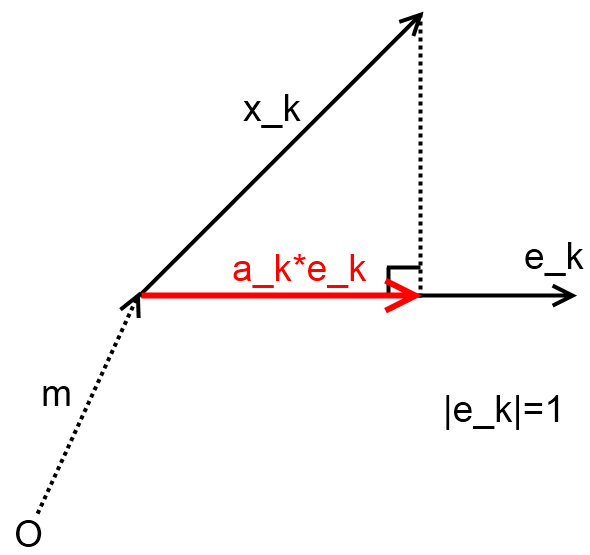
\includegraphics[width=5cm]{./images/principalComp.png}
  \end{minipage} 
  
  \skriptsubsubsection{Fisher Linear Discriminant}{117}
  \begin{minipage}{10.5cm}
  Very cool (according to Guido).
    \begin{aufzaehlung}
      \item Calculate the $d$-dimensional sample mean for every class
        $\bm{m}_i = \frac{1}{n_i} \sum\limits_{\bm{x} \in \mathcal{D}_i} \bm{x}$
      \item Obtain scatter matrices (= covariance matrix without division of N):
        $\bm{S}_i = \sum\limits_{\bm{x} \in \mathcal{D}_i} 
        (\bm{x}-\bm{m}_i) (\bm{x}-\bm{m}_i)^T$
        and the withing-class scatter matrix for the two-category case
        $\bm{S}_W = \bm{S}_1 + \bm{S}_2$
      \item Finding the Fisher linear discriminant:
        $\bm{w} = \bm{S}_W^{-1} (\bm{m}_1 - \bm{m}_2)$
        (normalize to$||\bm{w}||=1$.)
      \item Now we can transform and reduce dimensionality to a scalar:
        $y = \bm{w}^T \bm{x}$
    \end{aufzaehlung}
  \end{minipage}\hspace{5mm}
  \begin{minipage}{8cm}
    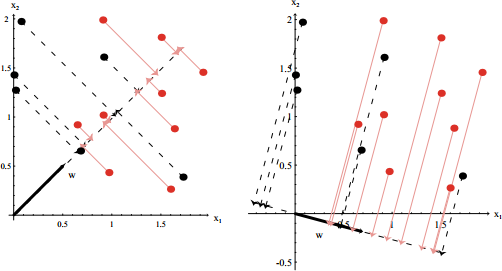
\includegraphics[width=8cm]{./images/fisher_discriminant.png}
  \end{minipage}
  
  \skriptsubsection{Hidden Markov Models}{128}
  \begin{minipage}{11cm}
    Hidden Markov Models (HMMs) are used to model timing dependencies, e.g.  
    in speech recognition the order of the characters.
    
    Problems:
    \begin{liste}
      \item Evaluation problem: Determine the \em probability \em that a particular sequence of 
      visible states $\bm V_T$ was generated by \em that model\em.
      \item Decoding problem: Determine the \em most likely sequence of hidden states \em $\bm \omega^T$ that
      led to observations $\bm V_T$.
      \item Learning problem: Given the structure and training observations, \em learn the parameters \em
      $a_{ij}$ and $b_{jk}$. 
    \end{liste}
    
    \skriptsubsubsection{Evaluation}{132}
      The Forward algorithm leads to $P(\bm V_T)$ and $\alpha_j(t)$. $\alpha_j(t)$ is the
      probability that the model is in state $\omega_i$ and has generated the target sequence up to step $t$.\\
      
      The Backward algorithm leads to $P(\bm V_T)$ and $\beta_j(t)$. $\beta_j(t)$ is the
      probability that the model is in state $\omega_j$ and the target sequence will be generated from step $t+1$ to the end $T$.
      
      
    \skriptsubsubsection{Decoding}{135}
      The Decoding algorithm from the book can return impossible solutions due to the fact that
      the $a_{ij}$ are not considered completely. Use the Viterbi decoder instead.
    
    \skriptsubsubsection{Learning}{137}
      The Forward-Backward (Baum-Welch) algorithm is an iterative algorithm which finds the HMM 
      weights $a_{ij}$ and $b_{ik}$ in a local optimum.
      \begin{aufzaehlung}
        \item Initialize $a_{ij}$, $b_{ik}$ with prior knowledge or uniformly distributed
        \item Loop start
        \item Use the Forward and Backward algorithms to find out $\alpha_i(t)$, $\beta_j(t)$ and $P(\bm V_T|\bm \Theta)$
        \item Calculate $\gamma_{ij}(t)$, $a_{ij} = \hat a_{ij}$, $b_{jk} = \hat b_{jk}$
        \item Restart loop when $a_{ij}$ and $b_{jk}$ didn't change a lot ($\delta_1$) or 
        $P(\bm V_T|\bm \Theta)$ didn't change a lot ($\delta_2$)
      \end{aufzaehlung}
      
  \end{minipage}\hspace{5mm}
  \begin{minipage}{8cm}
	\hspace{1cm}
    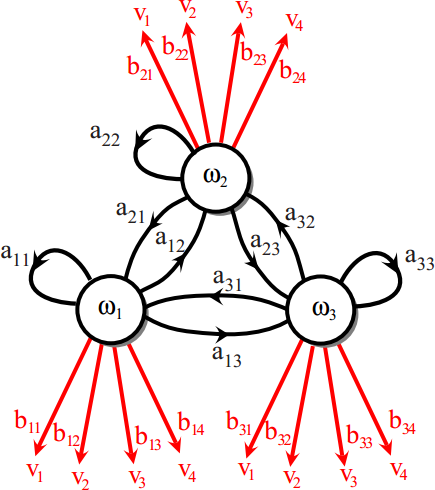
\includegraphics[width=5cm]{./images/hiddenMarkovModel.png}
    
    \begin{tabular}{ll}
      Hidden states              &$\omega_i$\\
      Absorbing/final state      &$\omega(T) = \omega_0$\\
      Visible states             &$\bm V_T = [v_1, \ldots, v_T]$\\
      Transition probability     &$a_{ij} = P(\omega_j(t+1) | \omega_i(t))$\\
      Emission probability       &$b_{jk} = P(v_k(t) | \omega_j(t))$\\
      $\sum\limits_j a_{ij} = 1$ &$\sum\limits_k b_{jk} = 1$\\
    \end{tabular}
    
    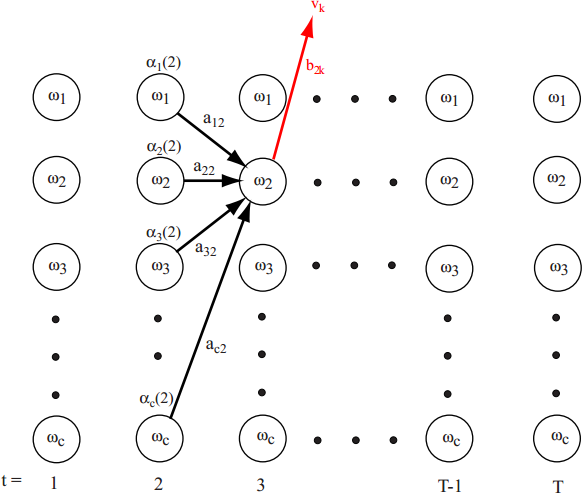
\includegraphics[width=7cm]{./images/hiddenMarkovModel2.png}
  \end{minipage}
  